\documentclass[twocolumn,twoside,letterpaper]{article} 

\usepackage{color}
\usepackage{caption}
\usepackage{subcaption}
\usepackage{geneticsT2}
\usepackage{times}
\usepackage{hyperref}

\addtolength{\oddsidemargin}{-.2cm}
\addtolength{\evensidemargin}{-1.2cm}
\addtolength{\textwidth}{1.5cm}
\addtolength{\topmargin}{-2cm}
\addtolength{\textheight}{3.5cm}

\renewcommand{\textfraction}{0.01}
\renewcommand{\topfraction}{0.99}
\renewcommand{\bottomfraction}{0.65}
\renewcommand{\floatpagefraction}{0.90}
\renewcommand{\dbltopfraction}{0.95}
\renewcommand{\dblfloatpagefraction}{0.80}
\renewcommand{\sfdefault}{phv}


% %%%
% % for latexml
% \usepackage{latexml}
% 
% % only do this stuff if latexml is not parsing the document
% \iflatexml
%   \renewcommand\sfbf[1]{\sf{\bfseries#1}}
% \else 
% % do this stuff:
\usepackage{fancyhdr}
\pagestyle{fancy}
\fancyhf{}

\fancyfoot[LE,RO]{{\sfbf \thepage}}
\renewcommand{\headrulewidth}{0pt}
\fancypagestyle{plain}{
	\fancyhf{}
}

%editing commands (please leave in for now)
\newcommand{\jri}[1]{\textcolor{blue}{ \emph{\scriptsize  #1}} }
\definecolor{gerkegreen} {rgb} {0,0.6,0}
\newcommand{\jpg}[1]{\textcolor{mattgreen}{ \em{\scriptsize  #1}} }

\usepackage[normalem]{ulem}
\def\dt{\bgroup
 \markoverwith{\lower-0.2ex\hbox
 {\kern-.03em\vbox{\hrule width.2em\kern0.45ex\hrule}\kern-.03em}}%
 \ULon}
\MakeRobust\dt
\usepackage[normalem]{ulem}
\def\dt{\bgroup
 \markoverwith{\lower-0.2ex\hbox
 {\kern-.03em\vbox{\hrule width.2em\kern0.45ex\hrule}\kern-.03em}}%
 \ULon}
\MakeRobust\dt
% ok latexml pay attention again
\fi

%%%%

\setcounter{footnote}{1}
%
%\title{The genomic impacts of drift and selection for hybrid performance in maize}
%Corresponding author:  Department of Plant Sciences, University of California, Davis, California 95616, USA. 
%    E-mail: \mbox{rossibarra@ucdavis.edu}}\\[0.3cm]
%   \small\sf $^{\ast}$Division of Plant Sciences, University of Missouri, Columbia MO 65211,\\
%   \small\sf $^\dag$Corn Insects and Crop Genetics Research Unit, USDA-Agricultural Research Service, Ames, IA, 50011\\
%   \small\sf $^\ddag$Plant Genetics Research Unit, USDA-Agricultural Research Service, Columbia MO 65211,\\
%   \small\sf $^\S$Department of Plant Sciences, The Center for Population Biology and the Genome Center, University of California, Davis, California 95616 , USA,\\
%   \small\sf $^1$ Present address:  DuPont Pioneer, Johnston, Iowa
%}
   %\small\sf  Present address: Graduate University for Advanced Studies, Hayama, Kanagawa 240-0193, Japan\\
%}

\title{Independent molecular basis of convergent highland adaptation in maize}
\author{
 \small\sfbf{Justin P. Gerke$^{\ast,1}$\thanks{
Corresponding author:  DuPont Pioneer, 8305 NW 62ND Ave, P.O. Box 7060
Johnston, IA, 50131   E-mail: \mbox{justin.gerke@gmail.com}}, Jode W. Edwards$^{\dag}$, Katherine E. Guill$^{\ddag}$, Jeffrey Ross-Ibarra$^{\S}$}\thanks{
Corresponding author:  Department of Plant Sciences, University of California, Davis, California 95616. 
    E-mail: \mbox{rossibarra@ucdavis.edu}},\\ 
\small\sfbf{and Michael D. McMullen$^{\ast,\ddag}$}\\[0.3cm]
   \small\sf $^{\ast}$Division of Plant Sciences, University of Missouri, Columbia MO 65211\\
   \small\sf $^\dag$Corn Insects and Crop Genetics Research Unit, USDA-Agricultural Research Service, Ames, IA, 50011\\
   \small\sf $^\ddag$Plant Genetics Research Unit, USDA-Agricultural Research Service, Columbia MO 65211\\
   \small\sf $^\S$Department of Plant Sciences, Center for Population Biology, and Genome Center, University of California, Davis, CA 95616  
}


 
%\date{Revised manuscript for \emph{Genetics}, \today}

\abstract{
 Modern maize breeding relies upon selection in inbreeding populations to improve the performance of cross-population hybrids. 
The United States Department of Agriculture - Agricultural Research Service (USDA-ARS) reciprocal recurrent selection experiment between the Iowa Stiff Stalk Synthetic (BSSS) and the Iowa Corn Borer Synthetic No. 1 (BSCB1) populations represents one of the longest standing models of selection for hybrid performance. 
To investigate the genomic impact of this selection program, we used the Illumina MaizeSNP50 high-density SNP array to determine genotypes of progenitor lines and over 600 individuals across multiple cycles of selection. 
Consistent with previous research (Messmer et al., 1991; Labate et al., 1997; Hagdorn et al., 2003; Hinze et al., 2005), we found that genetic diversity within each population steadily decreases, with a corresponding increase in population structure. 
High marker density also enabled the first view of haplotype ancestry, fixation and recombination within this historic maize experiment. 
Extensive regions of haplotype fixation within each population are visible in the pericentromeric regions, where large blocks trace back to single founder inbreds. 
Simulation attributes most of the observed reduction in genetic diversity to genetic drift. 
Signatures of selection were difficult to observe in the background of this strong genetic drift, but heterozygosity in each population has fallen more than expected. 
Regions of haplotype fixation represent the most likely targets of selection, but as observed in other germplasm selected for hybrid performance (Feng et al., 2006), there is no overlap between the most likely targets of selection in the two populations. 
We discuss how this pattern is likely to occur during selection for hybrid performance, and how it poses challenges for dissecting the impacts of modern breeding and selection on the maize genome. }


\usepackage{natbib}
\bibpunct{(}{)}{;}{a}{}{,}

\usepackage{amsmath}

\usepackage{graphicx}

\begin{document}

\maketitle

%%%%%%%%%%%%%%%%%%%%%%%%%%%%%%%%%%%%%%%%%% INTRO
\section*{Introduction}
Although maize is naturally an out-crossing organism, modern breeding develops highly inbred lines that are then used in controlled crosses to produce hybrids. Hybrid maize has been so successful that it quickly replaced long-standing mass-selected open pollinated varieties (Crabb, 1947). 
Maize inbred lines are now partitioned into separate inbreeding ‘heterotic groups’ that maximize performance and hybrid vigor (heterosis) when an inbred line of one group is crossed with the other group (Tracy and Chandler, 2006). 
The shift towards selection of inbred lines based on their ability to generate good hybrids – referred to as ‘combining ability’ – constituted an abrupt change from the open-pollinated mass selection that breeders practiced for millennia (Anderson, 1944; Troyer, 1999).
Multiple studies with molecular markers have indicated that the modern era of single-cross hybrid maize breeding has led to a dramatic restructuring of population genetic variation (Duvick et al., 2004; Ho et al., 2005; Feng et al., 2006). 
Different heterotic groups have diverged genetically over time to become highly structured and isolated populations. 
Advances in high throughput genotyping and the development of a maize reference genome now enable the observation of maize population structure at high marker density across the whole genome \citep{ganal2011a-large,chia2012maize}. 
So far, these high-density studies have examined a broad spectrum of germplasm at various points in the history of maize to search for the signals of population structure and artificial selection \citep{Hufford2012b, van2012historical}. 
Although selective sweeps remaining from domestication are clearly visible, the impact of selection during modern breeding appears comparatively small in terms of its impact on genomic diversity despite steady, heritable improvement in phenotype (Duvick, 2005). 
The lack of distinct selection signals from modern breeding may be due to specific selective events occurring in different populations, necessitating a more focused look within heterotic groups or even single breeding programs. 
In this study, we apply a genomic approach to study the dynamics of genetic variation over time within an individual selection experiment. 
The Iowa Stiff Stalk Synthetic (BSSS) and the Iowa Corn Borer Synthetic No. 1 (BSCB1) Reciprocal Recurrent Selection Program of the USDA-ARS at Ames, Iowa (hereafter referred to as the Iowa RRS) represents one of the best-documented public experiments on selection for combining ability and hybrid performance. 
BSSS and BSCB1 have been recurrently selected for improved cross-population hybrids (Penny and Eberhart, 1971). 
This model of selection, named reciprocal recurrent selection, provides the generalized model for strategies used in commercial maize breeding (Comstock et al., 1949; Duvick et al., 2004). 
The Iowa RRS experiment proves especially relevant because lines derived from the BSSS population have had a major impact upon the development of commercial hybrids (Duvick et al., 2004; Darrah and Zuber, 1986), the formation of modern heterotic groups (Troyer, 1999; Senior et al., 1998), and the choice of a maize reference genome \citep{schnable2009the-b73-maize}.
%%%%%%%%%%%%%%%%%%%%%%%%%%%%%%%%%%%%%%%%%% INTRO

\section*{Methods}
blah


\section*{Results}

%%%%%%%%%%%%%%%%%%%%%%%%%%%%%%%%%%%%%%%%%% FIGURE
\begin{figure}[tb]   
  \begin{center}
   \vspace{-0mm}
   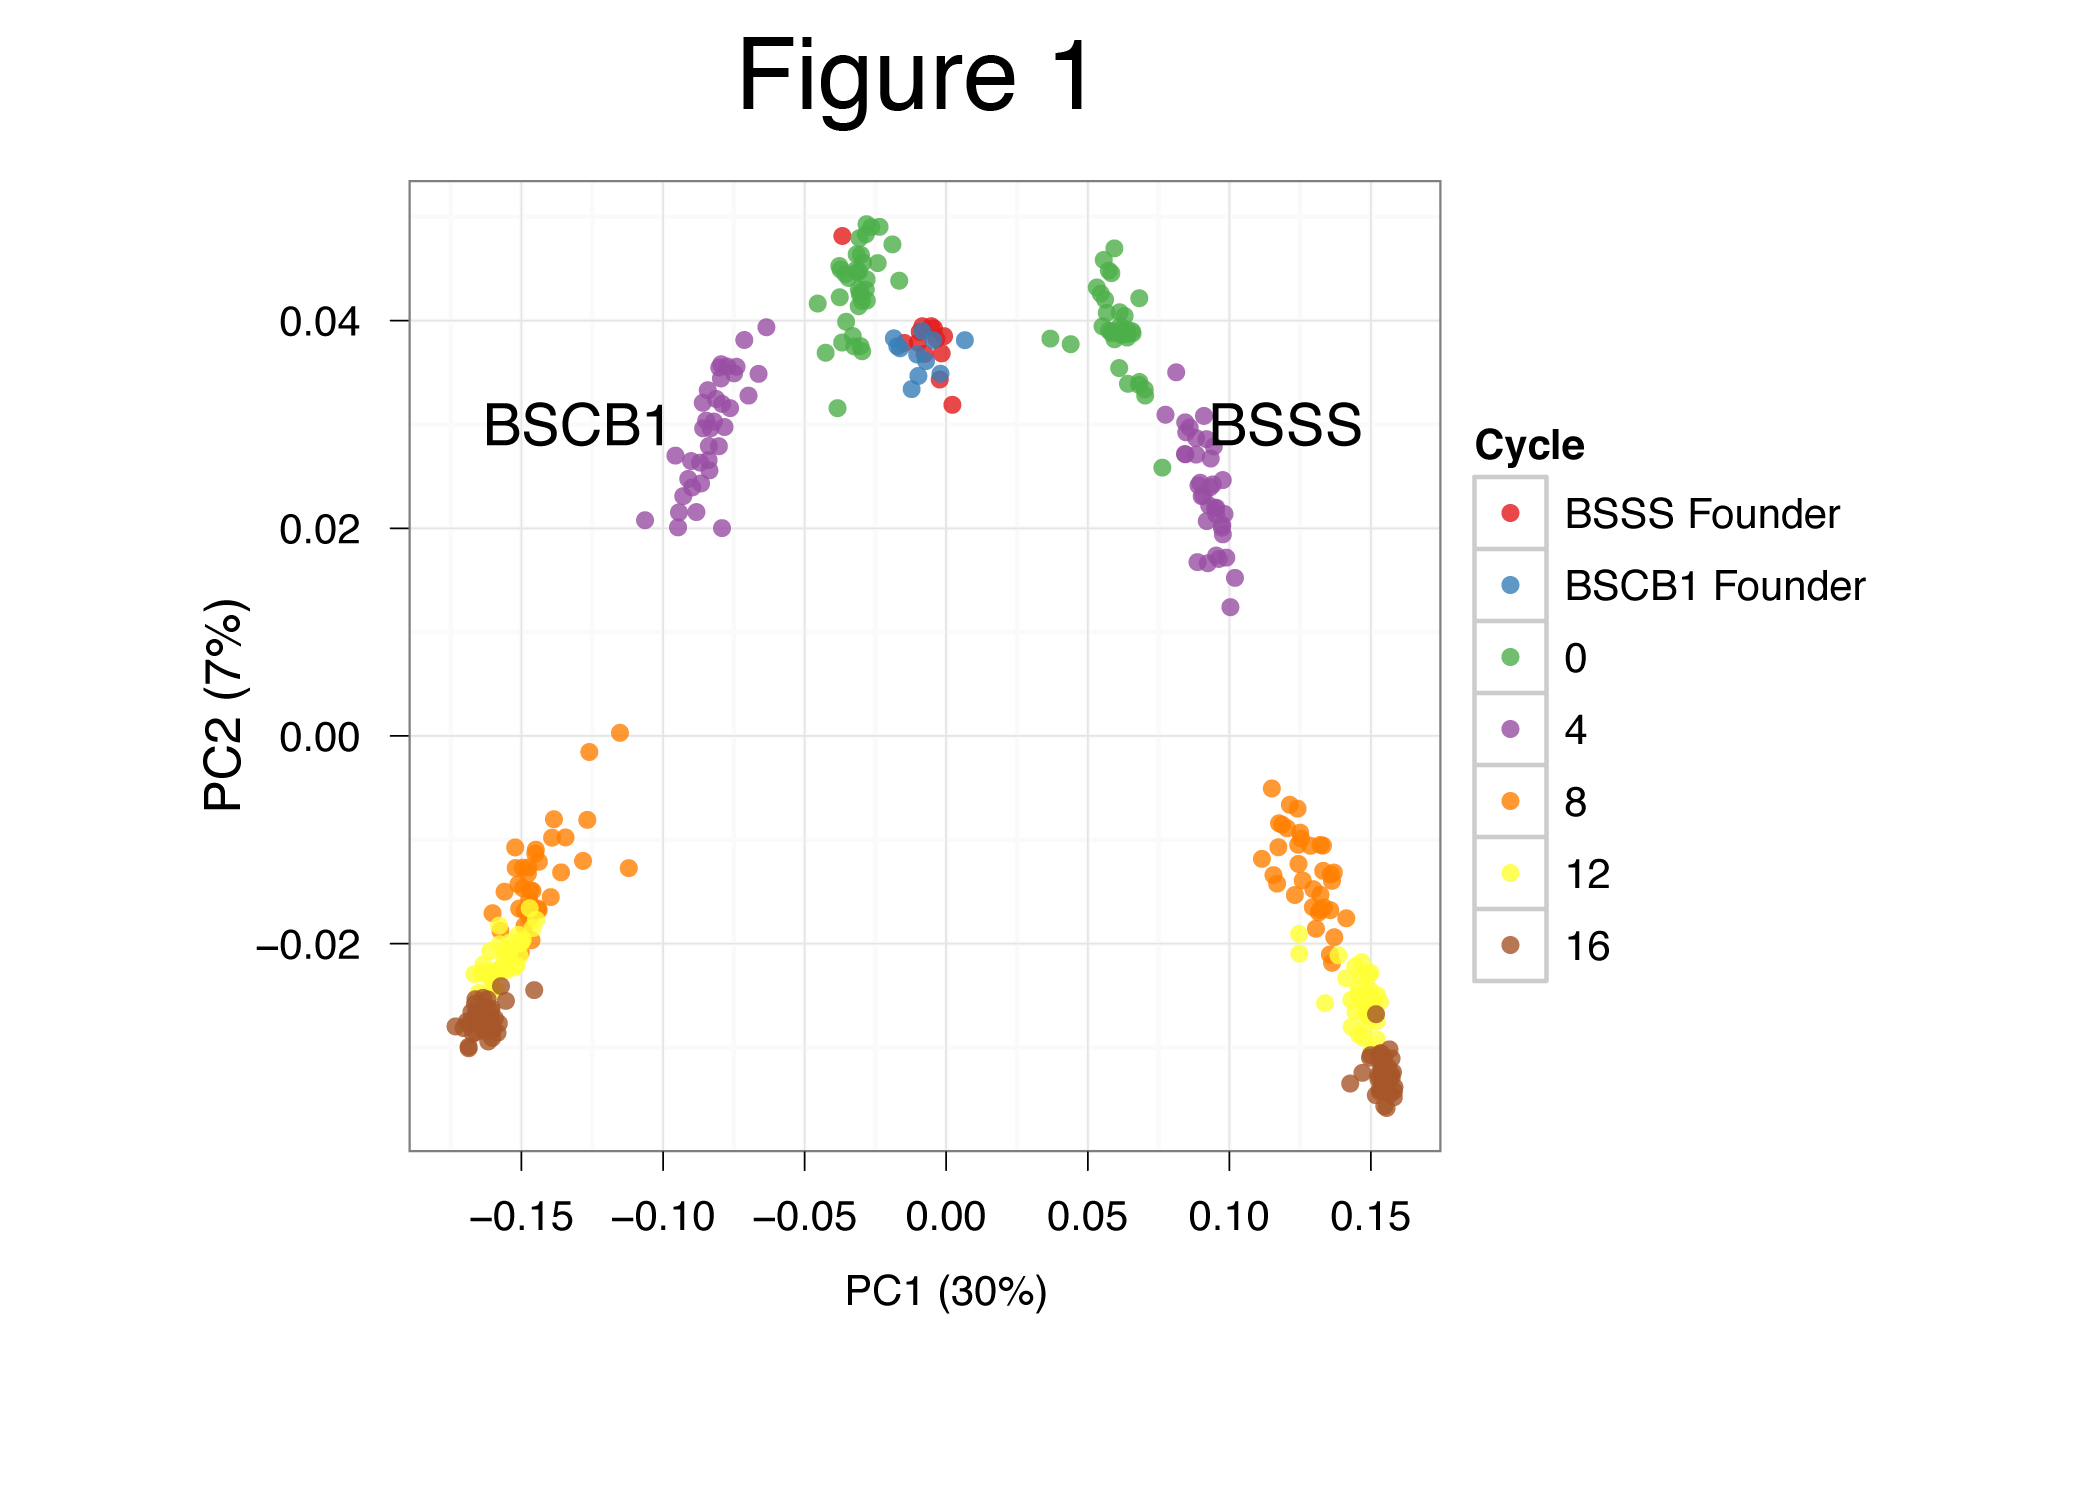
\includegraphics[width=0.4\textwidth]{fig1}
   \renewcommand{\baselinestretch}{0.9}
   \vspace{-3mm}
   \caption{BLAH} 
\vspace{-6mm}
    \label{fig:pca}
  \end{center}
\end{figure}
%%%%%%%%%%%%%%%%%%%%%%%%%%%%%%%%%%%%%%%%%% FIGURE

%%%%%%%%%%%%%%%%%%%%%%%%%%%%%%%%%%%%%%%%%% FIGURE
\begin{figure}[tb]   
  \begin{center}
   \vspace{-0mm}
   \includegraphics[width=0.4\textwidth]{fig2}
   \renewcommand{\baselinestretch}{0.9}
   \vspace{-3mm}
   \caption{BLAH} 
\vspace{-6mm}
    \label{fig:decline}
  \end{center}
\end{figure}
%%%%%%%%%%%%%%%%%%%%%%%%%%%%%%%%%%%%%%%%%% FIGURE

%%%%%%%%%%%%%%%%%%%%%%%%%%%%%%%%%%%%%%%%%% FIGURE
\begin{figure}[tb]   
  \begin{center}
   \vspace{-0mm}
   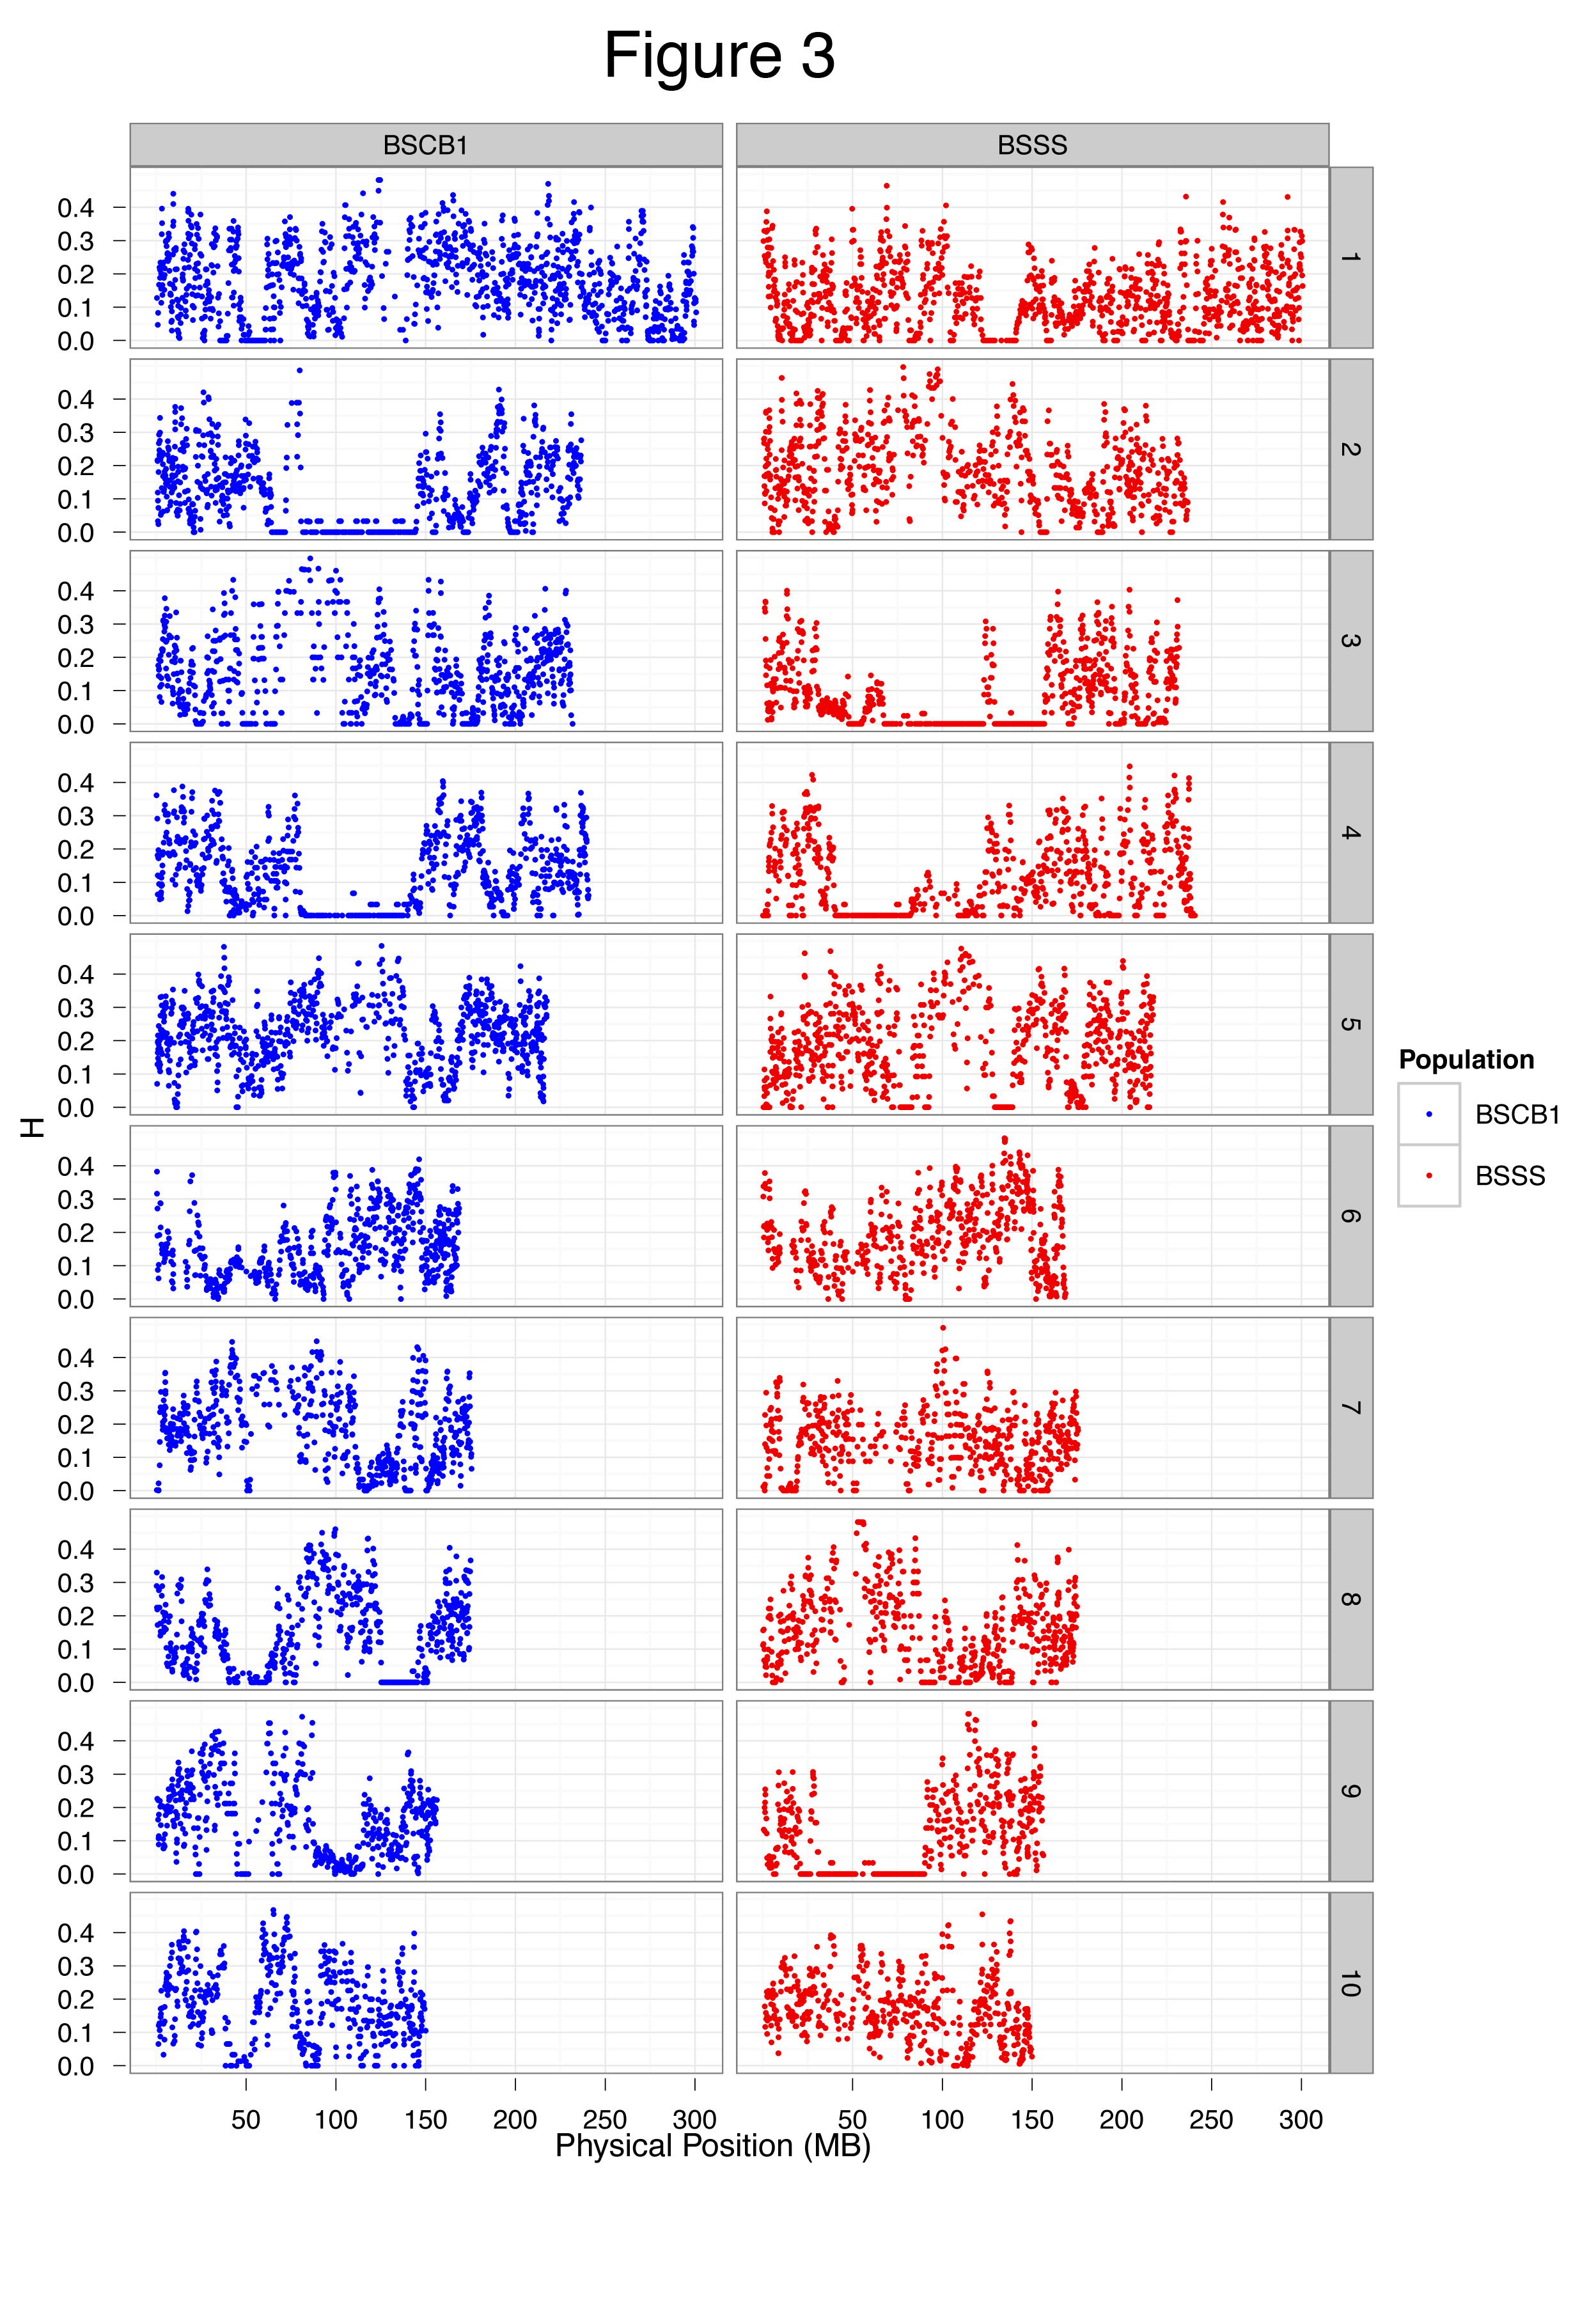
\includegraphics[width=0.4\textwidth]{fig3}
   \renewcommand{\baselinestretch}{0.9}
   \vspace{-3mm}
   \caption{BLAH} 
\vspace{-6mm}
    \label{fig:heterotic}
  \end{center}
\end{figure}
%%%%%%%%%%%%%%%%%%%%%%%%%%%%%%%%%%%%%%%%%% FIGURE

%%%%%%%%%%%%%%%%%%%%%%%%%%%%%%%%%%%%%%%%%% FIGURE
\begin{figure}[tb]   
  \begin{center}
   \vspace{-0mm}
   \includegraphics[width=0.4\textwidth]{fig4}
   \renewcommand{\baselinestretch}{0.9}
   \vspace{-3mm}
   \caption{BLAH} 
\vspace{-6mm}
    \label{fig:genphys}
  \end{center}
\end{figure}
%%%%%%%%%%%%%%%%%%%%%%%%%%%%%%%%%%%%%%%%%% FIGURE

%%%%%%%%%%%%%%%%%%%%%%%%%%%%%%%%%%%%%%%%%% FIGURE
\begin{figure}[tb]   
  \begin{center}
   \vspace{-0mm}
   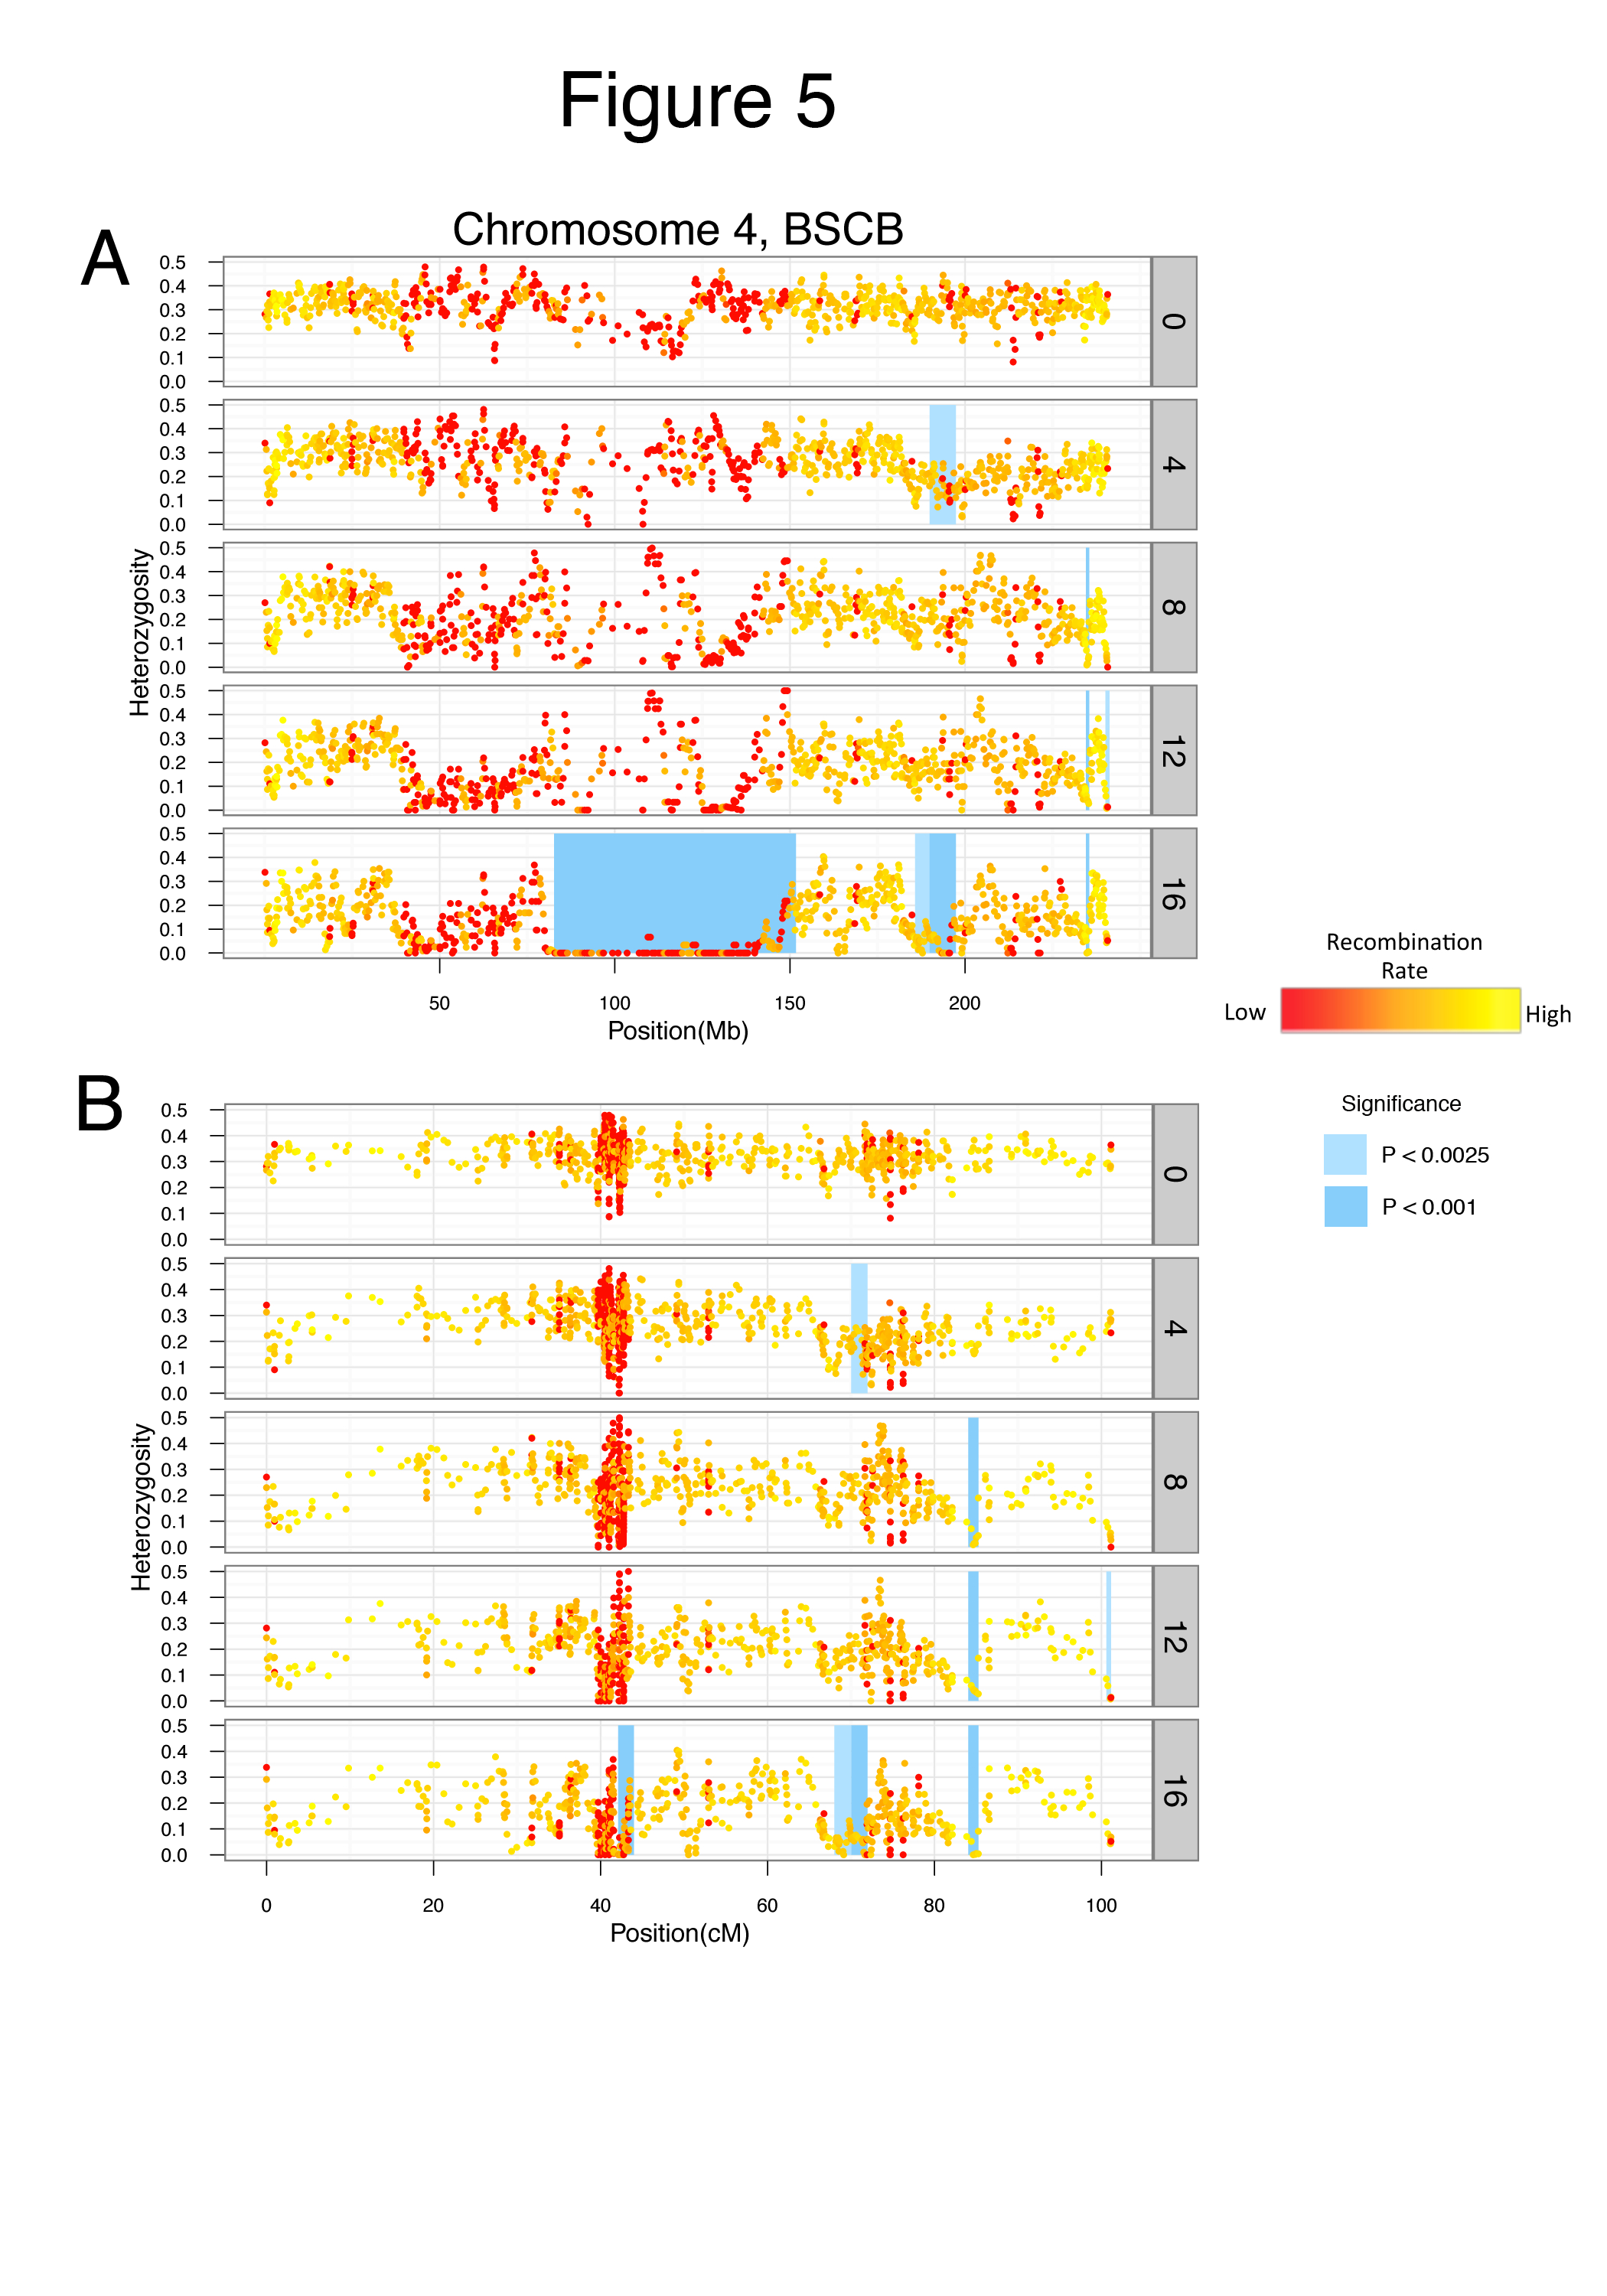
\includegraphics[width=0.4\textwidth]{fig5}
   \renewcommand{\baselinestretch}{0.9}
   \vspace{-3mm}
   \caption{BLAH} 
\vspace{-6mm}
    \label{fig:genphys2}
  \end{center}
\end{figure}
%%%%%%%%%%%%%%%%%%%%%%%%%%%%%%%%%%%%%%%%%% FIGURE

\section*{Discussion}
blah


\begin{acknowledgments}
We thank O. S. Smith and members of the Ross-Ibarra lab for comments on earlier versions of the manuscript. J.P.G received support for this research as a Merck Fellow of the Life Sciences Research Foundation. This research was supported by the National Science Foundation (IOS-0820619) and funds provided to USDA-ARS (MDM). Names of products are necessary to report factually on available data: however, neither the USDA, nor any other participating institution guarantees or warrants the standard of the product and the use of the name does not imply approval of the product to the exclusion of others that may also be suitable.
\end{acknowledgments}

\bibliography{references/references.bib}
\bibliographystyle{geneticsT2}

%\suppl



%%%%%%%
% put supplemental figures and tables here:
% e.g.
% \begin{figure}
% ...


%%%%%
% appendices to follow
%\input{HighLowSup1} 

\end{document}

